\chapter{Sampling and A/D conversions}
\section{Impulse response} \label{sec:impulseresponse}
	In order to analyse time invariant linear systems an useful analyses is the one of the \de{impulse response} $h(t)$ (in the continuous time case, while $h(n)$ for the discrete one) defined as 
	\begin{equation}
		h(\cdot) = T\big\{ \delta(\cdot) \}
	\end{equation}
	where $T$ is the expression that relates the input $x$ with the output $y$ of the system. Depending on the nature and the behaviour of the response we can classify the systems, and in particular in the continuous time case we have that $h(t)$ has an infinite duration, while in the discrete time we can have both have \textit{infinite impulse response} IIR or \textit{finite impulse response} FIR systems.
	
	We analyse the impulse response because it permits to fully describe the system and compute the outputs for every generic input signal. Given in fact a linear time invariant LTI system, then 
	\[ \forall x(\cdot) \qquad \Rightarrow \quad y(\cdot) = x(\cdot) * h(\cdot) \]
	and so the output can be calculated as a convolution.
	
	\begin{proof}
		In the discrete time case this relation can be proven considered the sequence of input pulses $x(n)$ that can be rewritten as
		\[ x(n) = \sum_{k=-\infty}^\infty x(k)\, \delta(n-k) \]
		Computing the output of the system given  it's transformation using $T$, and considering the linearity property we can see that
		\[ y(n) = T \left\{ \sum_{k=-\infty}^\infty x(k)\, \delta(n-k)  \right\} = \sum_{k=-\infty}^\infty x(n) T\big\{ \delta (n-k) \big\} \]
		Considering that the system is also time invariant this means that the response $T\big\{ \delta (n-k) \big\} = h_k(n-k)$ is constant and so
		\[ y(n) = \sum_{k=-\infty}^\infty x(k) h(n-k) = x(n) * h(n) \]\vspace{3mm}
		
		A continuous time signal $x(t)$ can instead be rewritten as
		\[ x(t) = \lim_{\tau\rightarrow0} \sum_{k=-\infty}^{\infty} x(k\tau) \rect_\tau(t-k\tau) \]
		Similarly to the discrete time case we can evaluate the response of the linear time invariant system as
		\begin{align*}
			y(t) & = \lim_{\tau\rightarrow0} T\left\{ \sum_{k=-\infty}^{\infty} x(k\tau) \rect_\tau(t-k\tau) \right\} = \lim_{\tau\rightarrow0} \sum_{k=-\infty}^{\infty} x(k\tau) T \left\{ \frac 1 \tau \rect_\tau(t-k\tau) \right\}\tau 
		\end{align*}
		Geometrically the function $\frac 1 \tau \rect_\tau(t-k\tau)$ represent a rectangle whose area is always one, and in particular having $\tau\rightarrow 0$ the function tends to the dirac pulse: the response $T\left\{\frac 1 \tau \rect_\tau(t-k\tau)\right\}$ can so be considered as the impulse response $h_\tau(t-k\tau)$ of the system.
		\[ y(t) = \lim_{\tau\rightarrow0} \sum_{k=-\infty}^{\infty} x(k\tau) h_\tau(t- k\tau) \tau = \intinf x(\tau) h(t-\tau)\, d\tau = x(t)*h(t)  \]
	\end{proof}
	
	An important thing to consider is the frequency response of the system by transforming the impulse response, and so $H(\cdot) = \four{h(\cdot)}$ represent the \de{frequency responses} of the linear time invariant system; the magnitude $|H(\cdot)|$ can be referred as \textbf{magnitude response} while $\angle H(\cdot)$ is the \textbf{phase response} of the system.
	
	Because $h(\cdot)$ is a real function, due to the properties of the Fourier transform we can state that $|H(\cdot)|$ presents a even symmetry (on the frequency axes) while $\angle H(\cdot)$ is an odd function. 
	
	Considering also that the output can be computed as the convolution of the impulse response with the input in the time case, then the frequency response of the output can be calculated as
	\begin{equation}
		Y(\cdot) = H(\cdot) X(\cdot)
	\end{equation}
	
\section{Filters}
	A \de{filter} is (typically) a linear system selective in the frequency axes that determines which frequencies should be accepted and the one that should be removed. In general is possible to observe 4 kind of \de{ideal filters} (considering the magnitude response principally):
	\begin{itemize}
		\item \textbf{low-pass filter} that accepts magnitudes $|H(\Omega)|$ only for $\Omega < \Omega_c$ while it cancels all the other values. This filter can be modelled as a rectangle function with module 1 in the range $[-\Omega_c,\Omega_c]$;
		\begin{center}
			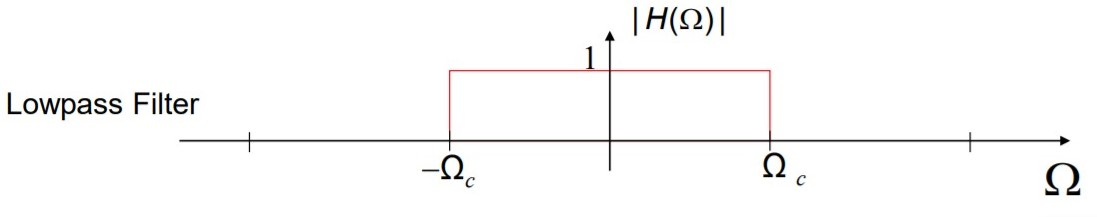
\includegraphics[width=9cm]{filter-low}
		\end{center}
		
		\item the dual behaviour is performed by the \textbf{high-pass filter} that allows to pass through the system only frequencies above a value $\Omega_c$;
		\begin{center}
			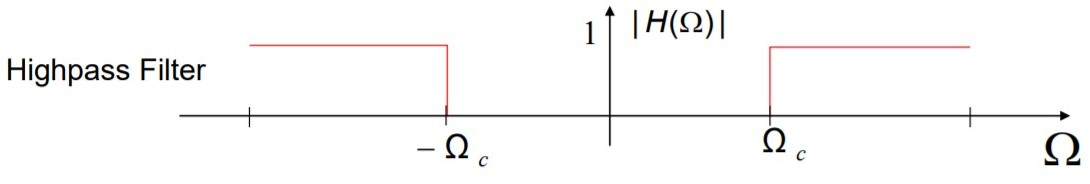
\includegraphics[width=9cm]{filter-high}
		\end{center}
		
		\item \textbf{band-pass filters} are useful to select only a band of frequencies and so allowing only a range $[\Omega_a,\Omega_b]$ of frequencies to be transmitted.
		\begin{center}
			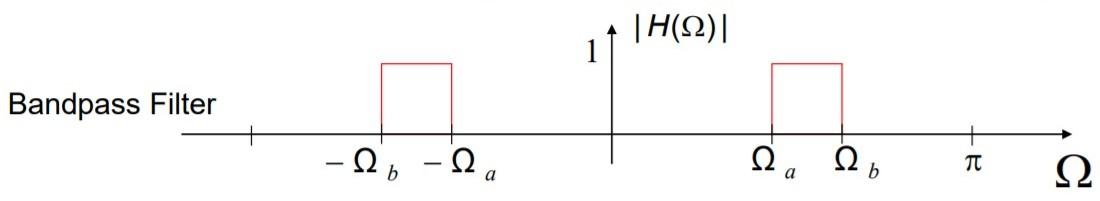
\includegraphics[width=9cm]{filter-band}
		\end{center}
		
		The dual case is the \textbf{stop-band filter} that blocks the frequencies in the specified range.
	\end{itemize}
	All this filters are ideal because in  the real world is impossible to implement this kind of response, but only can approximate them and this is due to the causality of the systems (to implement ideal system we need to know also the future behaviour of the signal).
	
\section{Ideal continuous - discrete conversion}
	The \de{analog to digital conversion} ADC process implies the \de{sampling} (of period $T_s$) of a continuous time signal $x_c(t)$ in order to convert it in a discrete time sequence $x(n)$ (that still an analog signal, it's just a discretization on the time axes of the original signal). In the ideal case the output sequence $x(n)$ can be rewritten as
	\begin{equation}
		x(n) =x_c\big(nT_s\big) = x_c(t) \infsum \delta\big(t-nT_s\big)  
	\end{equation}
	Considering that $\delta\big(t-nT_s\big)$ is a periodic function we can use the Fourier series (with the complex notation) and so
	\begin{align*}
		x(n) & = x_c(t) \infsum c_n e^{j\frac{2\pi}{T_s}nt} \qquad \leftarrow c_n = \frac 1 {T_s} \four{\delta(t)}\Big|_{n} = \frac 1 {T_s} \\
		&= \frac{x_c(t)}{T_s} \infsum e^{j\frac{2\pi}{T_s}nt}
	\end{align*}
	Let's consider now to apply the Fourier transform on this signal substituting $n = -k$ we can determine that
	\begin{equation}
		\four{x_c(nT_s)} = X_c(\Omega) * \frac 1 {T_s}\sum_{k=-\infty}^\infty \delta\left(\Omega- \frac{2\pi}{T_s}k\right) = \frac{1}{T_s} \sum_{k=\infty}^\infty X_c\left(\Omega - \frac{2\pi}{T_s}n \right)
	\end{equation}
	This represent the ideal definition of the frequency spectrum of a sampled signal. In particular we can note that the spectrum of the signal is the exact infinite replica of the continuous spectrum $X_c(\Omega)$ with the spectral replicas distances by a value $\frac{2\pi}{T_s}$, as shown in figure  \ref{fig:conv:replicas}.
	
	\begin{figure}[bht]
		\centering
		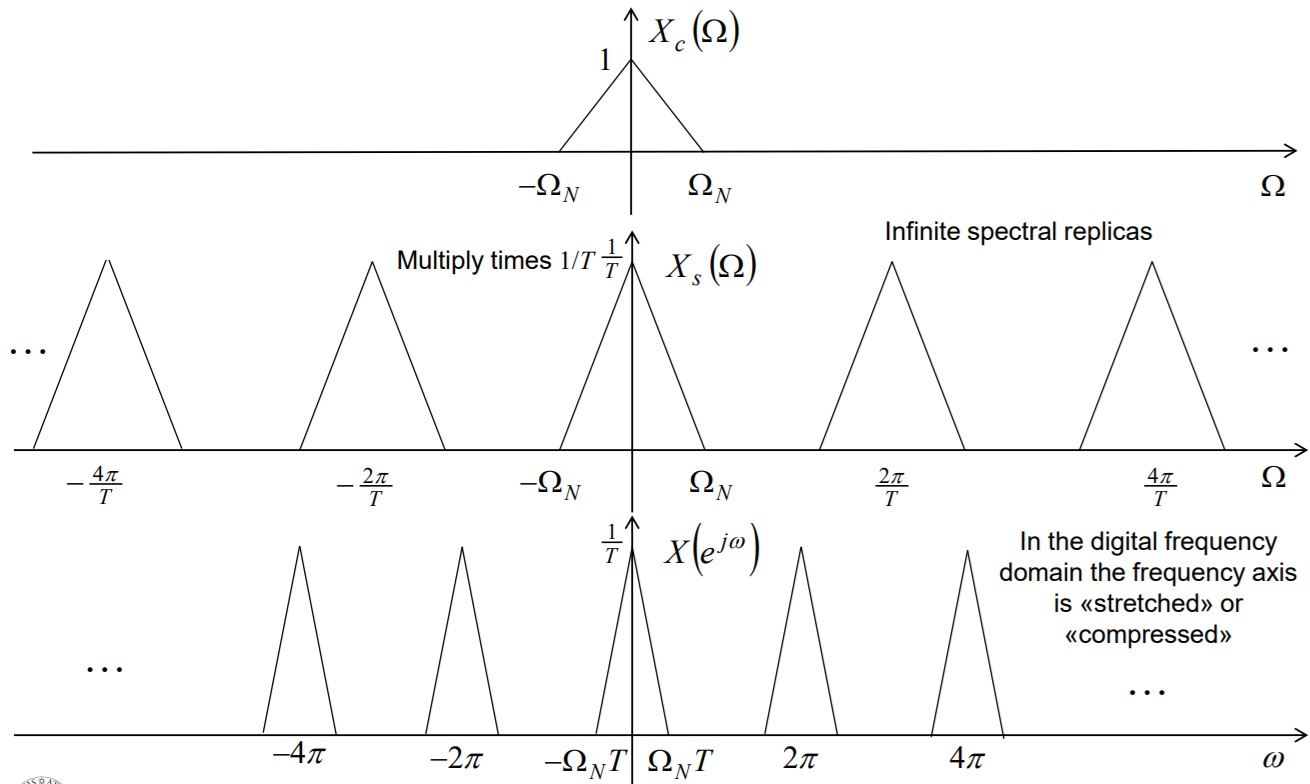
\includegraphics[width=\linewidth]{replicas}
		\caption{from above: frequency spectrum $X_c(\Omega)$ of the signal $x_c(t)$, frequency spectrum of the sampled signal $x(nT_s)$ for the continuous time Fourier transform and then the spectrum $X(e^{j\omega})$ considering the discrete time Fourier transform.} 
		\label{fig:conv:replicas}
	\end{figure}
		
	Considering $x(nT_s)$ as a discrete time signal $x(n)$ we have a re-scalation of the time axes and determine an identical spectrum that doesn't depend on the sampling period $T_s$. Considering that $\Omega T = \omega [rad]$ we have a relation that's independent from the time and so is more a \textit{digital} definition. We can so use the discrete Fourier transform
	\[ x(n) \quad \mapsto \quad X(e^{j\omega})\]
	and by representing the spectrum (figure \ref{fig:conv:replicas}) the replicas are now at multiples of $2\pi$ (having rescaled the axes of a factor $T_s$).
	
	\subsection{Nyquist sampling theorem}
		The \de{aliasing} problem arise when the spectral replicas of the signals (due to the sampling) tends to overlap and happens when the sampling period is to high (or the sampling frequency is too low in respect to the frequencies of the signal). When this happens that we lose too much information from the original signal and so it's impossible to reconstruct it in an acceptable manner. 
		
		\begin{example}{: sampling of a sine wave}
			Let's consider a sine wave of period $T_0$, if we consider a sampling period $T \ll T_0$ than we can observe that having a lot of samples allows us to \textit{decompose} with good approximation the original sine wave, while considering a sampling period $T \backsim T_0$ than most of the information are lost and the constructed signal isn't good enough.
		\end{example}
		
		The aliasing problem must always be avoided because the loss of information is irrecoverable and in order to do so we have to decrease the sampling period $T_s$ (increasing the sampling frequency $f_s$) in order to avoid the overlap of replicas. Given the maximum frequency $\Omega_n$ of the spectrum of the signal in order to avoid aliasing we have to make sure that
		\[ \Omega_n < \frac \pi {T_s} \]
		This represent the base of the \de{Nyquist Shennon sampling theorem}: determining in fact the frequency $f_n = \Omega_n/2\pi$ we can state that
		\begin{equation}
			2\pi f_n < \pi t_s \qquad \Rightarrow \quad f_n < \frac{f_s}{2} \quad \leftrightarrow \quad \omega_n < \pi
		\end{equation}
		and so the signal frequency should always be less then half of the sampling frequency. In particular we refer to $f_s/2$ as the \de{Nyquist frequency} and determines the maximum allowable frequency of the input signal in order to not have aliasing.
		
	\subsection{Sample \& hold}
		To implement a real analog-digital converter we have to consider the continuous-discrete time converter that's preceded by an \de{anti aliasing filter} $H_a(\Omega)$, a low-pass filter that stops frequencies above the Nyquist one in order to avoid (or at least reduce) the aliasing problem.
		
		Consequently to the sampler we need to have a \de{ZOH} Zero Order Hold filter that allows to put a constant output and refresh the out (setting it equals to the input) every sampling period $T_s$ in order to allow the proper ADC to perform correctly his operation; this step should also avoid the \textit{shocking} of the transients associated to the switch commutations. To complete the description of the analog-digital conversion we also need a quantizer block (to discretize the analog function in the values range) and an encoding block that determines a digital output. 
		
		\begin{figure}[bht]
			\centering
			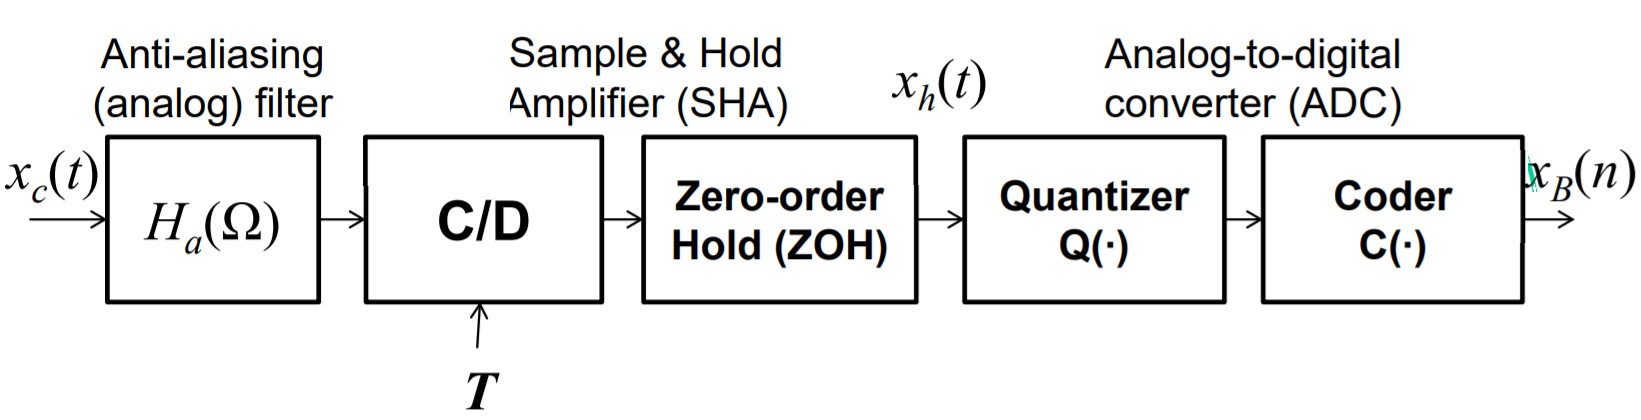
\includegraphics[width=10cm]{adc-steps}
			\caption{composing block of a analog digital converter unit.}
		\end{figure}
		
		In a practical way the operation of continuous to discrete conversion and zero order hold filter is done by the circuit called \de{simple \& hold amplifier SHA} modelled as in figure \ref{fig:conv:samplehold}.
		
		\begin{SCfigure}[2][bht]
			\centering
			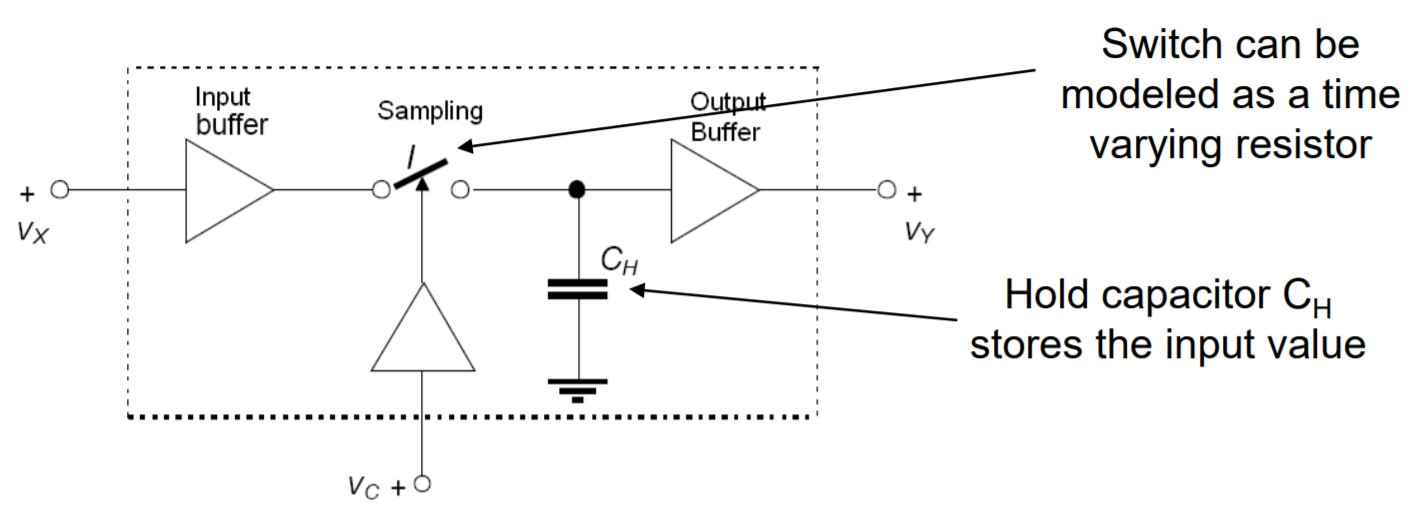
\includegraphics[width = 8cm]{samplehold}
			\caption{possible implementation of an electrical sample\&hold amplifier. }
			\label{fig:conv:samplehold}
		\end{SCfigure}
	
		This kind of circuit implementation resembles a low pass electrical filter; ideally while the sampling signal $v_c$ is one them the exit $v_y$ is equal to the input voltage $v_x$, while when $v_c=0$ the exist remains constant (hold operation) due to the constant charge of the capacitor. The time necessary to charge the capacitor $C_h$ is ideally negligible, but in reality we have to considered that  the on time should allow to charge the capacity in order to avoid spectral distortions. In real world application we have also to take into account that $C_h$ will discharge naturally over time due to parasitic currents.\\
		While designing this circuit we have to choose a $C_h$ value that's a trade off: low values of $C_h$ decrease the time required to charge the capacitor but also increase the current leak (it discharges quickly).
		
\section{Quantization and codification}
	At this point, with a sample \& hold amplifier, we have a constant sample for a time $T_s$ and it's signal is passed to the quantizer block that, in combination with the coder, determines the proper \textbf{analog to digital} converter.
	
	The \textbf{quantizer} block is used to discretize the signal value into a specified set of values that can be consequently \textbf{coded} into a digital signal. By an electrical point of view this operations are usually performed together.	
	
	While quantizing, given a range $[V_{min},V_{max}]$ of the input signal we can divide this range into separate intervals $I_k = (T_{k-1},T_k]$ (where $T_k$ is the $k$-th quantization threshold value on the horizontal axis) that's related to a code bin $Q_k$ wide $T_k - T_{k-1}$. We refer to \textbf{quantization levels} the \textit{response} of the stair-case function to the input (so measured on the vertical axis).
	
	\begin{SCfigure}[2][bht]
		\centering
		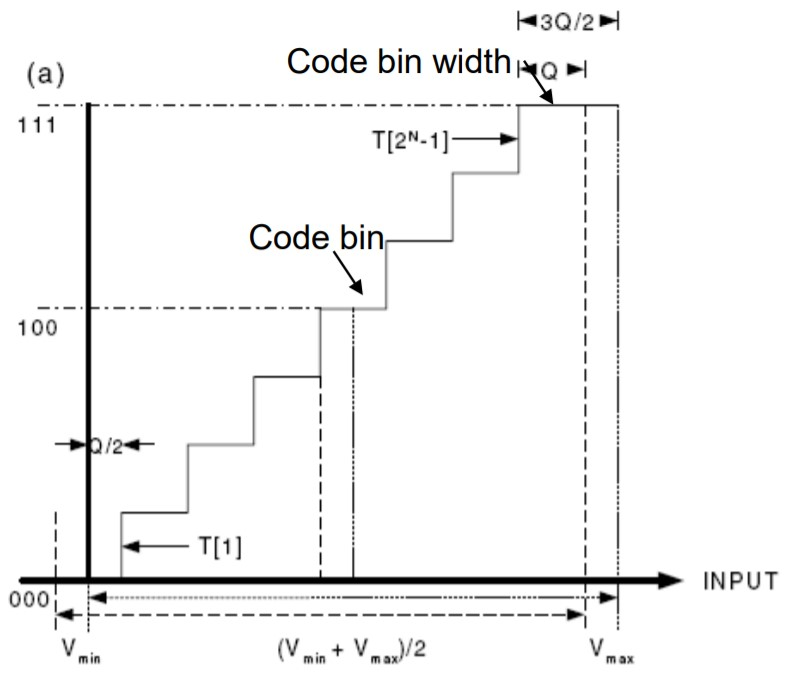
\includegraphics[width=6cm]{quantization}
		\caption{graphical representation of the stair-case function that determine the quantization of a signal.}
	\end{SCfigure}
	
	The quantization level is of course related to the digital implementation of the system: given a $b$ bits system the number of levels (equals to the digital combination of the signal) allowed are $2^b$. This means that the quantization thresholds have to be $2^b-1$.  
	
	If the range of quantization is symmetric (like $[-F_s,F_s]$) than the quantizer is called \textbf{bipolar}; we refer the system as \textbf{unipolar} when the quantization happens only for positive voltages as $[0,F_s]$. In general we consider uniform quantization steps.

	Considering that the quantization step $\Delta$ can be computed as
	\[ \Delta = \begin{cases}
		\frac{2F_s}{2^b} = \frac{F_s}{2^{b-1}} \qquad & \textrm{bipolar} \\
		\frac{F_s}{2^b} & \textrm{unipolar}
 	\end{cases} \]
 	and so the resolution is exponentially related to the bit number used to code the signal.
 	
 	\begin{SCfigure}[2][bht]
 		\centering
 		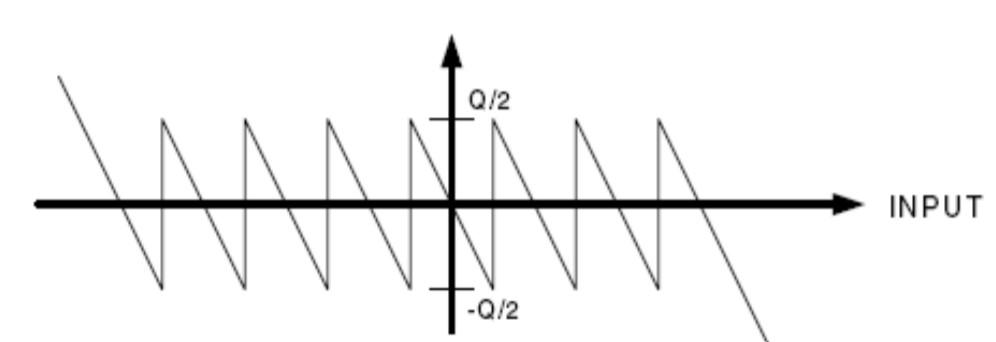
\includegraphics[width=6cm]{quanterror}
 		\caption{quantization error computed as the difference between the real value and the quantized one considering a rounding system.}
 	\end{SCfigure}
	
	The error of the quantization has a range of maximum $\Delta$ and we can have a rounding system (the quantization error $e_q$ is spaced in the range $[-\frac \Delta 2, \frac \Delta 2]$) or a truncated/flooring one (where $e_q \in [0,\Delta]$). This quantization error is a random process and it's a matter of modelling of the quantizer block. Considering in fact that the quantizer block $Q(\cdot)$ is a non linear system, all the theory studied until now collapses and can lead to instabilities in the random processes; however usually the error $e_q$ is small (considering that the number of bits $b$ is increasing, lowering so $\Delta$) and so it can be neglected. With this assumption the quantization error can be considered as a strict sense stationary random process assumed as a white noise with correlation $C(x(t),e_q(t)) = 0$ negligible and with a probability density function with a uniform distribution:
	\[ f(e_q) = \begin{cases}
		\rect_{\Delta}(0) \qquad &\textrm{rounding} \\
		\rect_{\Delta}(\Delta/2) \qquad &\textrm{truncation} 
	\end{cases} \]
	
	Considering the error $e_q$ as a  random process we can compute it's mean value $\mu_e$, variance $\sigma_e^2$ and power $P_e$ as
	\begin{align*}
		\mu_e &= 0 &\sigma_e^2 &= \frac{\Delta^2}{12} & P_e =  \frac{\Delta^2}{12} &  &&\textrm{rounding} \\
		\mu_e &= -\frac{\Delta}{2} & \sigma_e^2 &= \frac{\Delta^2}{12} & P_e =  \frac{\Delta^2}{3} &  &&\textrm{truncation} 
	\end{align*}
	We can see that the power of a truncation system is 4 times as large as the power of the rounding counterpart.
	
	\paragraph{Signal-to-noise and quantization ratio} The \textbf{signal-to-noise and quantization ratio} $SQNR$ (usually expressed in decibel) is a parameter that allows to compare the variance of the quantization error respect to the original signal and so
	\[ SQNR := \frac{P_x}{P_e}  \quad \xrightarrow[\textrm{rounding}]{dB} \quad 10 \log_{10}\left(\frac{\sigma_x^2}{\sigma_e^2}\right) = 10 \log_{10}\left( \sigma_x^2 \frac{3}{F_s^2}2^{2b} \right)\]
	\[ \Rightarrow \quad SQNR_{dB} \approx 6.02b + 20 \log_{10} \sigma_x + 20 \log_{10}\left(\frac{\sqrt 3}{F_s} \right) \]
	This means that for each bit $b$ added on the quantization level, the potential improvement of signal-to-noise ratio if of about $6dB$. In general, in order to have a proper number of bits (to have a low quantization error) we can consider the expression
	\begin{equation}
		b = \frac 1 2 \log_2 \left(\frac{\sigma_x^2}{\sigma_e^2}\right)
	\end{equation}
		
	In general the original signal $\hat x$ can be described by a quantized signal $x$, and error $e_q$ due to quantization, and error $e_\omega$ due to external noises and ADC imperfection and so
	\[ \hat x(n) = x(n) + e_q(n) + e_\omega(n) \qquad \Rightarrow \quad SNR = \left(\log_2 \frac{\sigma_x^2}{\sigma_e^2+\sigma_\omega^2}\right) < SQNR \]
	where $SNR$ is the \de{signal noise ratio} and consider all the errors as a uncorrelated noises (modelled so as white) that's more gaussian distributed than uniform. The fact that the two noise sources $e_q,e_\omega$ are statistically independent, then while computing the $SNR$ we can simply add the two variances (because their correlation is zero). In this case the $ENOB$, the \de{effective number of bits}, can be computed as
	\begin{equation}
		ENOB = b_e = \frac 12 \log_2 \frac{\sigma_x^2}{\sigma_e^2+\sigma_\omega^2}
	\end{equation}
	In general an ADC can be constructed with a $16bit$ quantization, but if the $ENOB$ (that depends on the frequency) is lower (like $12bit$), then the last significant bits (in this case $4bit$) are \textit{meaningless} because they are affected by the ADC noises.
		
\section{Technology implementations of ADC's}
	In general analog to digital converters are classified in categories depending on their technology implementation and the performance that they can achieve. In general for high resolution, the sample rate is low, while if the samples needed are very high, the resolution drops. As a rule of thumb when decreasing the nominal resolution by a bit, the sampling frequency that can be achieved doubles.
	
	\begin{SCfigure}[1][bht]
		\centering
		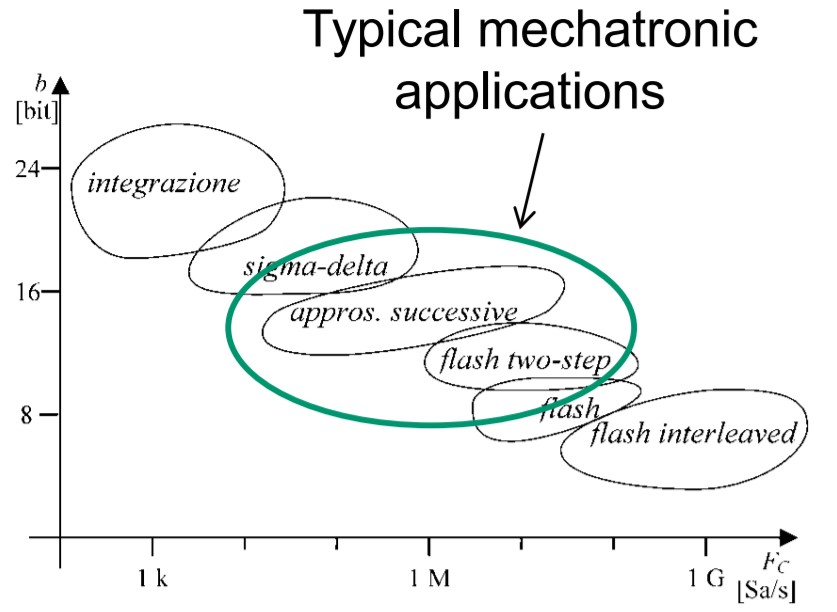
\includegraphics[width=6.5cm]{adc-families}
		\caption{families of analog to digital converters with associated performance as sample per second ($x$ axis) and resolution bits ($y$ axis).}
	\end{SCfigure}

	In mechatronics applications usually are used successive approximations ADC (or one with similar properties) because they have the best trade-off in terms of frequency and resolution.
	
	\subsection*{Flash ADC}
		The \de{flash ADC} is the fastest family of analog to digital converter and, as we can see in figure \ref{fig:conv:flash}, it consists in 3 main stage: the first determined by the resistor, the second composed by synchronized comparators and the last digital codification section.
		
		\begin{SCfigure}[2][bht]
			\centering
			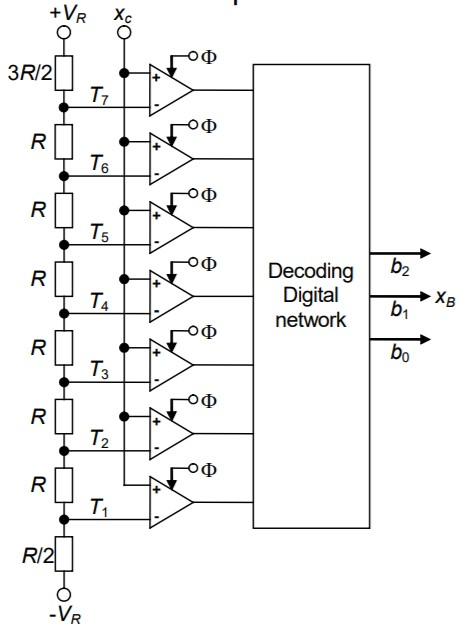
\includegraphics[width=4cm]{flash-adc}
			\caption{implementation of a $3bit$ flash analog to digital converter.}
			\label{fig:conv:flash}
		\end{SCfigure}
		
		
		Referring to the figure $V_r$ and $-V_r$ are the $F_s$ and $-F_s$ till now defined. $T_i$ are representing the various voltage threshold (due to the fact that the series of resistor determines a voltage divider). The first resistor (and the last) has a value of $R/2$ due to have a rounding ADC (and not a truncation one): in fact we can see that the $0$ value threshold is in the middle of the quantization range as we can see in figure \ref{fig:conv:flashsteps}. $\Phi$ is the signal that enable the comparator (if not active the output is fixed).
		
		\begin{SCfigure}[1][bht]
			\centering 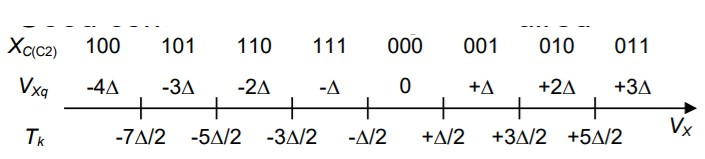
\includegraphics[width=7cm]{flash-adc-range}
			\caption{ideal quantization of the flash analog to digital converter.}
			\label{fig:conv:flashsteps}
		\end{SCfigure}
		
		This kind of implementation limits the resolution of the ADC (as number of bits $b$) because the number of required comparator (and the digital codification logic) is equal to $2^b-1$. This kind of implementation also present a high power consumption and increasing the resolution the uncertainties sources become predominant in the conversion itself.
		
\section{Digital to analog converter}
	In the ideal case the \textit{black box} that determines the conversion is just a pure reconstruction of the discrete signal in the continuous domain. Defining $y(n)$ as the discrete sequence to be reconstructed to a continuous signal $y_c(n)$ given a constant time $T_s$ then we can see that
	\[ Y(\Omega) = Y(e^{j\Omega T}) = \frac 1 T \sum_{k=-\infty}^\infty Y_c\left(\Omega - \frac{2\pi k}{T}\right) \]
	We can see that, as for the analog to digital conversion, the reconstructed spectrum of the signal present the copies with multiplicity $2\pi/T$. In this case for reconstructing a signal it's important to introduce an ideal low-pass reconstruction filter $H_r$ defined as
	\[ H_r(\Omega) = \begin{cases}
		T \qquad & |\Omega|\leq \frac \pi T \\ 0 & \textrm{otherwise}
	\end{cases} \qquad \Rightarrow \quad Y_c(\Omega) = H_r(\Omega) Y(\Omega) \]
	Representing the result in the time domain we can see that
	\begin{equation}
	\begin{split}
		y_c(t) & = \frac 1 {2\pi} \int_{-\pi/T}^{\pi/T} T \, Y(\Omega) e^{j\Omega t}\, dt = \frac T{2\pi}  \int_{-\pi/T}^{\pi/T} \left(\infsum y(n) e^{-j\Omega nT} \right) e^{j\Omega t}\, dt \\ & = \infsum y(n) \frac T{2\pi} \int_{-\pi/T}^{\pi/T} e^{j\Omega(t-nT)}\, d\Omega \\
		& = \infsum y(n) \, \sinc\left( t - nT \right)
	\end{split}
	\end{equation}
	With this expression it's possible to see that $y_c(n)$ is made just of the $n$-th component of the discrete value $y(n)$. In general we can see that the digital to analog conversion is kind of interpolation of the original signal as a cardinal sine function.
		
	\paragraph{Real digital to analog converter} Considering a real implementation of a digital to analog converter we must introduce a zero order hold filter between the decoder and the low pass reconstruction filter; in general the decodification and the ZOH are typically implemented together. \\
	The decoder is used to transform a digital binary number into a corresponding voltage. The zero order hold filter is instead used to re-introduce the concept of time from a discrete sequence of binary codes (in fact the time distance between this digital signals is unknown).
		
	\begin{SCfigure}[2][bht]
		\centering 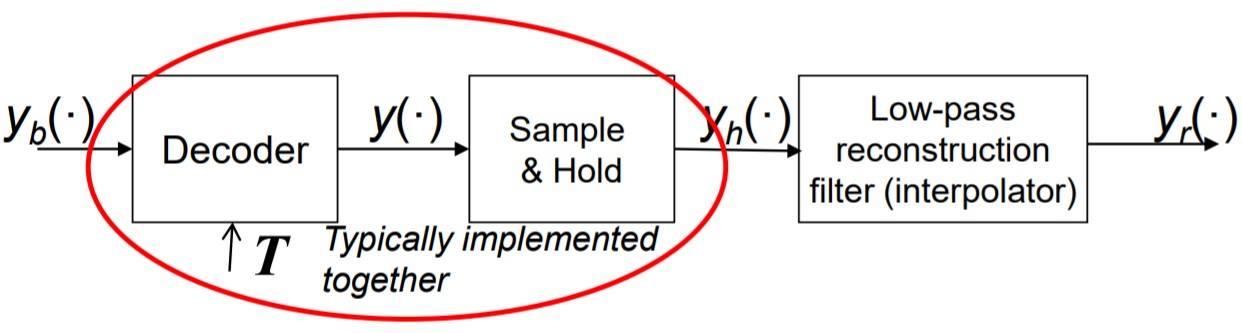
\includegraphics[width=8cm]{DAC-scheme}
		\caption{section that usually determines a digital to analog converter.}
	\end{SCfigure}

	Considering that $y_h(t)$ is the signal out of the sample and hold filter, the result is a staircase function that can be regarded as
	\begin{align*}
		y_h(t) & = \infsum y(n) \,\rect_T\left(t-\frac T2 - nT\right) = \infsum y_c(nT) \,\rect_T\left(t-\frac T2 - nT\right) \\
		& = y_c(t) \left[ \rect_T\left(t-\frac T2\right)*\infsum \delta(t-nT) \right]
	\end{align*}
	The representation of this signal in the frequency domain can be described as
	\begin{align*}
		Y_h(\Omega) & = Y_c(\Omega) * \left[ T \sin \left(\frac{\Omega T}{2}\right) e^{-j\Omega \frac T2} \cdot \frac 1 T \sum_{k=-\infty}^\infty \delta\left(\Omega - \frac{2\pi k}{T}\right) \right] \\
		& = \underbrace{\frac 1 T \sum_{k=-\infty}^\infty \delta\left(\Omega - \frac{2\pi k}{T}\right)}_{= Y(\Omega) = Y\left( e^{j\omega} \right) } T \,\sinc\left( \frac{\Omega T}{2} \right) e^{-j\Omega \frac T2} \\
		& = Y(\Omega) T\, \sinc \left(\frac{\Omega T}2\right) e^{-j\Omega \frac T 2} 
	\end{align*}
	The zero order hold is used so to reconstruct the signal (but it introduce some distortions) while steal attenuating the spectral replicas. Considering that this filter introduces an attenuation at the end of the required frequency, that introduces the fact that the low pass reconstruction filter can be less ideal with less stiffer transients. In reality to compensate for the ZOH error the filter should be
	\[ \hat H_r(\Omega) = \begin{cases}
		\frac{T}{H_h(\Omega)} \qquad & |\Omega| \leq \frac \pi T \\ 0 & \textrm{otherwise}
	\end{cases} \]
	
	\subsection{Technology implementations}
		In case of digital to analog converter there is less variety of components and so implementations families. An example is the \textbf{binary weighted voltage} DAC that uses $n$ resistor in parallel with ratio between successive components of $\frac 1 2$ that are all inputs of an inverting amplifier (constructed with the op-amp) that sums the necessary values. Considering that the current $I_n$ through the $n$-th resistor is
		\[ I_n = \frac{V_r}{R / 2^{n-1}} \]
		and so the output voltage is equal to
		\[ V_{out,i} = \frac{-R_r}{R_{i}} V_{i} \qquad \Rightarrow \quad V_{out, tot} =  - R_r \frac{V_r}{R} \sum_{n=1}^b b_n 2^{n-1} \]
		
		\begin{SCfigure}[2][bht]
			\centering 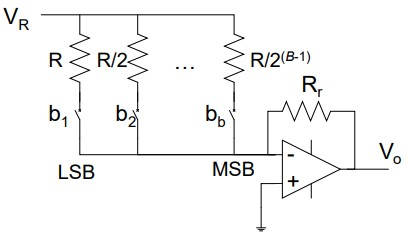
\includegraphics[width=5cm]{binary-dac}
			\caption{general implementation of a binary-weighted voltage digital to analog converters.}
		\end{SCfigure}
		
		The problem of this implementation is that building (with precision) the values of resistor between $R$ and $R/2^{b-1}$ (considering the exponential law) and so the number of bits is limited to $6-8$.		A solution to this problem is by using a \textbf{R-2R ladder network} DAC as in figure \ref{fig:conv:r2r}.
		
		\begin{SCfigure}[1][bht]
			\centering 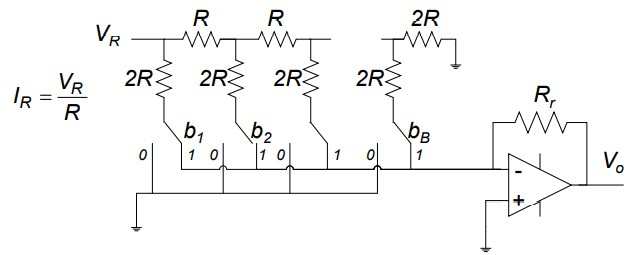
\includegraphics[width=6cm]{r-2r}
			\caption{implementation of a R-2R ladder network digital to analog converter.}
			\label{fig:conv:r2r}
		\end{SCfigure}
		
		For every stage we can see that the equivalent resistor $R_{eq}$ is equal to $2R$ and so every section is a perfect current divider of a value 2: every node bisect so the current.
		
		\begin{SCfigure}[2][bht]
			\centering 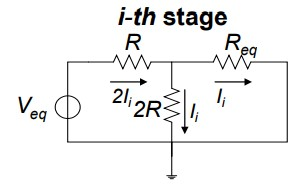
\includegraphics[width=4cm]{r-2r-stage}
			\caption{$i$-th stage of the R-2R ladder network DAC.}
		\end{SCfigure}

\section{Multi rate signal processing}
	Until now we referred to signal conversion with constant sampling frequency $f_s = 1/T_s$, but in general it's possible to have a variable value, and in this case we refer to the \de{multi rate signal processing}; in particular in this section we analyse signals subjected to
	\begin{itemize}
		\item \textbf{undersampling} (also associated to the \textit{decimation}), so when the new sampling period $T_s'$ is a multiple of the original sampling period
		\[ T_s' = M T_s\qquad M\in\mathds N \]
		\item \textbf{upsampling} when the new sampling period is a fraction of the starting value and so
		\[ T_s' = \frac{T_s}{L} \qquad L \in \mathds N \]
	\end{itemize}
	
	\paragraph{Undersampling (decimation)} Performing an undersampling (or similarly a decimation) determines that for a digital time signal $x(n)$, only one sample out of $M$ is chosen and so determines the new sequence $x_d(n)$ such that
	\[ x_d(n) = x(nM) \]
	In block diagrams this operation is done by the \textit{compressor} (figure \ref{fig:conv_compressor}).
	\begin{SCfigure}[2][bht]
		\centering 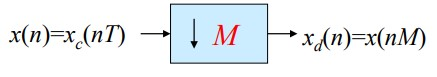
\includegraphics[width=6cm]{compressor}
		\caption{compressor as block diagram for describing an undersampling.} \label{fig:conv_compressor}
	\end{SCfigure}
	 
	The spectral representation of the undersampled signal is related to the original one and in fact we can see
	\begin{align*}
		X_c' (\Omega) = X_d\left(e^{j\omega T_s'}\right) & = \frac 1 {T_s'} \sum_{k=-\infty}^\infty X_c\left(\Omega - \frac{2\pi k}{T'_s}\right) \\
		& = \frac{1}{MT_s}\sum_{k=-\infty}^\infty X_c\left( \Omega - \frac{2\pi k}{MT_s} \right)	
	\end{align*}
	In the first line we can see that the undersampled signal can be considered as a standalone transform of the original continuous time signal $x_c$, however considering the second line we can see the relation with the transform of the signal with sampling period $T_s$: in fact the decimated signal presents replicas that rescales each with a factor $1/M$ on the frequency axis. In general undersampling a signal is like doing a brand new conversion with a different sampling period $T_s'$ that determines a new spectrum (and in this case the spectral replicas can be closer and introduce the phenomena of aliasing.)
	\begin{SCfigure}[2][bht]
		\centering 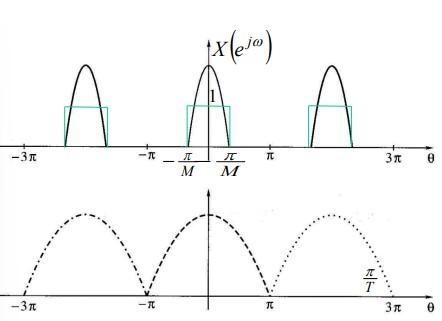
\includegraphics[width=6cm]{downsampling}
		\caption{original spectral response of a signal sampled with period $T_s$ (upper) and response of the signal considering an undersampling with $M=2$ (down).}
	\end{SCfigure}

	This principles are demonstrated for real evaluated signals, however the same can be said for the discrete time fourier transform where in fact the spectral replicas are placed every $\omega = 2\pi$:
	\[ X_d(e^{j\omega}) = \frac 1 {MT_s} \sum_{k=-\infty}^\infty X_c\left( \frac{\omega}{MT_s} - \frac{2\pi k}{MT_s}\right) \]
		
	In general the consequence of undersampling is a loss of information and that can lead to the aliasing problem (but in same cases this operation has a functional use).
		
	Combining the compressor with previously a low pass filter with cut-off frequency at $\omega_c = \pi/M$ (in order to avoid the aliasing) determines the block diagram of the \textbf{decimator}.	
	
	\paragraph{Upsampling (interpolation)} Considering an initial sequence $x(n)$, simply increasing the sampling period $T_s'$ (to have an upsampling) by a factor $L$ (respect to $T_s$) it means that we need to add new samples (in order to add new information) that in general means adding a value of zero in each new samples generated. After this operation we want to perform an interpolation to modify this zero values into a \textit{more correct} value of the sampled signal considering (as the name suggest) an interpolation.
		
	In block diagram the upsampling is represented by the expander (to create the upsampled signal with the zeros) and a low pass filter that does the work of the interpolator.
		\begin{SCfigure}[2][bht]
			\centering 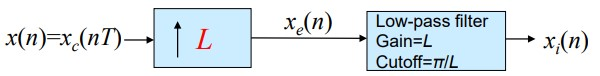
\includegraphics[width=6cm]{upsampling}
			\caption{block diagram representation to do an upsampling by using an expander and an interpolator.}
		\end{SCfigure}
	
	With this representation we can note that the expanded signal $x_e$ can be described as
	\[ x_e(n) = \begin{cases}
		x(n/L) \qquad &n = 0,\pm L,\pm 2L,\dots \\ 0 & \textrm{otherwise}
	\end{cases} \]
	and so by computing the discrete time fourier transform we obtain
	\begin{align*}
		X(e^{j\omega}) &= \frac 1 {T_s} \sum_{k=-\infty}^\infty X_c\left(\frac \omega {T_s} - \frac{2\pi k}{T_s}\right) \\
		X_e(e^{j\omega}) &= \infsum x_e(n) e^{-j\omega n} = \sum_{k=-\infty}^\infty x(n) e^{-j\omega k L} = X(e^{j\omega '}) \\
		& = \frac 1 {T_s} \sum_{k=-\infty}^\infty X_c \left( \frac{\omega'}{T_s} - \frac{2k\pi}{T_s} \right) = \frac 1 {LT_s'} \sum_{k=-\infty}^\infty X_c \left( \frac{\omega}{T_s'} - \frac{2\pi k}{LT_s'} \right)
	\end{align*}
	where $\omega' = L \omega$. From the graphical point of view, the original sampled sequence and the upsampled one presents the same magnitude but the spectral replicas are no longer located at a distance $T_s$, but at a value $T_s/L$ and the replicas are compressed by a factor $L$.
		\begin{SCfigure}[2][bht]
			\centering 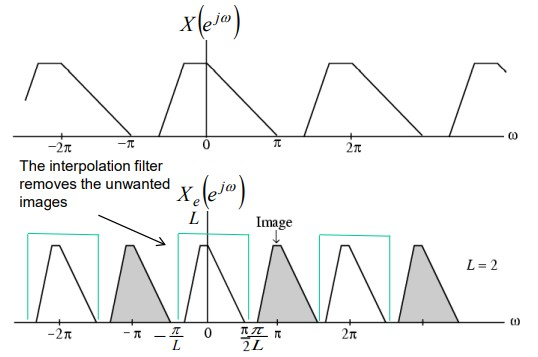
\includegraphics[width=6cm]{upsampling-graph}
			\caption{original spectrum due to the sampling of a signal (upper) and upsampled spectrum (bottom) of the same signal with a value $L=2$.}
			\label{fig:conv:upsampling}
		\end{SCfigure}
	
	In general the difference between the upsampled signal and a pure sampling with period $T_s'$ is that $X_e$ has a magnitude reduces by a factor $L$ and present in a frequency range of $2\pi/T_s'$ presents $L$ spectrum replicas (while the pure sampled signal would have presented just one replica). As we can see in figure \ref{fig:conv:upsampling}, the presence of the interpolator block that deletes the unwanted replicas of the spectrum due to the upsampling, so the grey replicas. In order to do this operation correctly interpolator should be a low pass filter with a gain of $L$ and a cut-off frequency of $\pi/L$.
	
	In the time domain the ideal interpolation relies on a noncausal $\sinc$ function, in fact
	\[ h_i(n) = \frac{\sin\left( \frac{\pi n}{L}\right)}{\frac{\pi n}{L}} \]
	The simplest method to achieve the goal of a good interpolation is using a linear filter one as described in figure \ref{fig:conv:lininterp}
	
	\begin{SCfigure}[2][bht]
		\centering 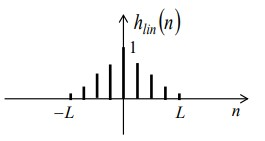
\includegraphics[width=5cm]{lin-interp}
		\caption{time response of a linear interpolator.} \label{fig:conv:lininterp}
	\end{SCfigure}
	
	
	
	
	
	
	
	
	
	
	
	
	
	
	
	
	
	
	
	
	
	
		
		
	
	
	
	